\documentclass[12pt,a4paper]{report}
\usepackage{amssymb,amsthm,amsmath,amscd}
\usepackage{latexsym}
\usepackage{enumerate}
\usepackage[german]{babel}
\usepackage{verbatim}
\usepackage[hyphens]{url}
\usepackage{hyperref}
\usepackage[utf8]{inputenc}
\usepackage{pdfpages}
\usepackage{graphicx}
\usepackage{csquotes}
%\usepackage[landscape]{geometry}
\begin{document}
\begin{titlepage}
	\begin{center}

		\vspace*{1.0cm}
		\huge
		\textsc{\bf{PS Algorithmen für verteilte Systeme}}

		\vspace*{4.0cm}
		\textsc{
			\normalsize{eingereicht von} \\[0.5\baselineskip]
			{\large Baumgartner Dominik, Dafir Samy}
		}

		\vspace*{3.0cm}
		\textsc{
			\normalsize{Gruppe  1(16:00)}
		}

	\end{center}
\end{titlepage}

\section*{Aufgabe 17}
Es wurden der Clockwise, wie auch der Radius Growth Algorithmus implementiert. Beide wählen einen Leader in einem Ring-Netzwerk mit 10000 Knoten.
Beide Algorithmen wurden auf 100 verschiedenen Graphen ausgeführt und Runden- sowie Nachrichten- und Hopanzahl ausgewertet.
Im folgenden werden die Ergebnisse dargestellt und analysiert.
\subsection*{Clockwise}
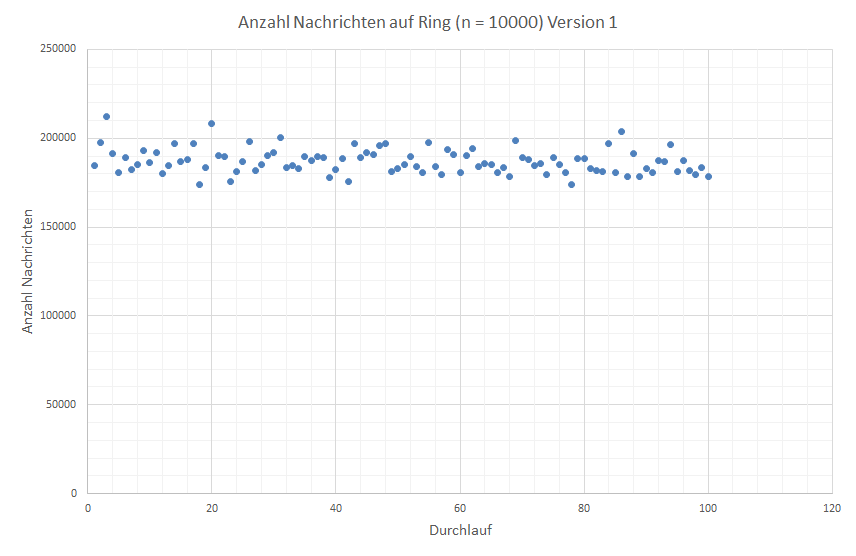
\includegraphics[width=\textwidth]{cw-1.png}
Der Clockwise Algorithmus verhält sich wie in der VO beschrieben und weist damit auch die erwartete Runden- und Nachrichtenanzahl auf.\\
Rundenanzahl: $O(n)$\\
Schritte: $O(n)$\\
Nachrichten: $O(n^2)$\\
In unserem Setup ergab sich eine Hop- bzw. Rundenanzahl von 10000. Die Nachrichtenanzahl wurde im Plot dargestellt.
Da aus der Formulierung des Algorithmus nicht eindeutig hervorgeht, ob Knoten, die noch keine Nachricht mit größerer ID erhalten haben,
in jeder Runde die eigene ID senden, wurden 2 Versionen ausgewertet. In ersterer senden Knoten ihre eigene ID weiter, bis eine
größere ID erhalten wurde. Da es unserer Meinung nach keinen Sinn macht, die eigene ID mehr als einmal zu senden, wurde eine zweite Version getestet, in der die eigene ID nur einmal gesendet und dann erst wieder etwas gesendet wird, wenn eine größere ID erhalten wurde.\\
Wie erwartet wirkte sich die Änderung positiv auf die Anzahl der gesendeten Nachrichten aus, ohne dabei die korrekte Leaderwahl zu
beeinflussen. die Nachrichtenanzahl wird auf etwas mehr als die Hälfte reduziert.\\
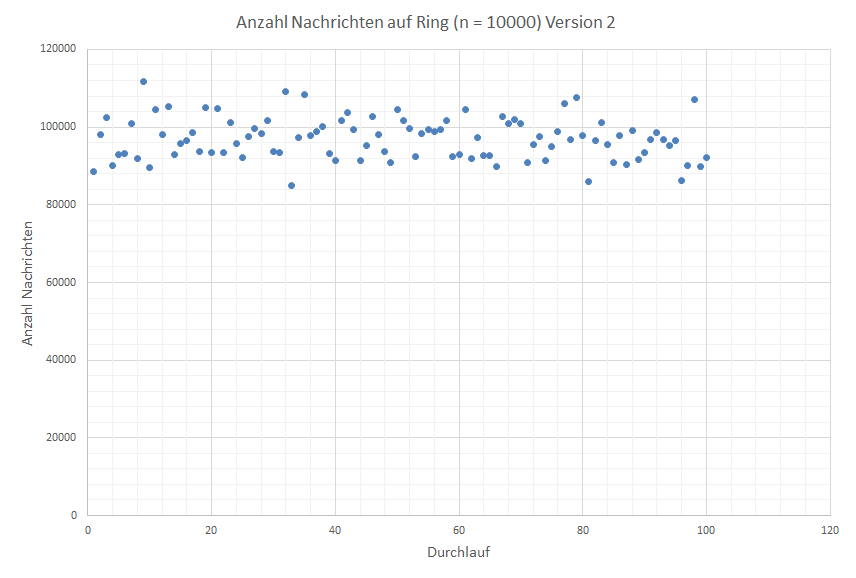
\includegraphics[width=\textwidth]{cw-2.png}
\subsection*{Radius Growth}
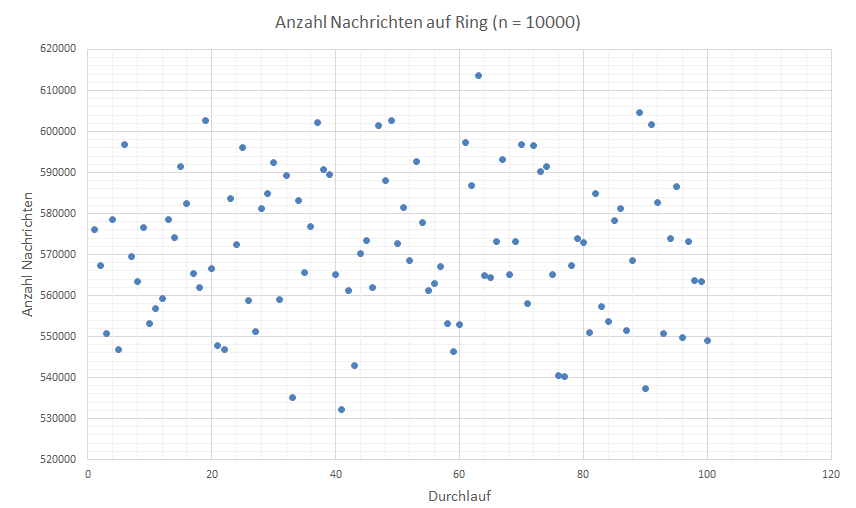
\includegraphics[width=\textwidth]{rg.png}
Auch der Radius Growth Algorithmus verhält sich wie erwartet und weist foolgende Runden- bzw. Nachrichtenanzahlen auf.\\
Rundenanzahl: $O(log(n))$\\
Schritte: $O(n)$\\
Nachrichten: $O(n*log(n))$\\
In unserem Setup erhielten wir eine Hopanzahl von 52766, sowie eine Rundenanzahl von 15. Die Rundenanzahl kommt aufgrund des
exponentiellen Wachstums der TTL zustande. Da in Runde 15 $TTL = 2^{14} = 16384$ ist, ist dies die letzte Runde, da sich der Sender mit
der größten ID in dieser Runde selbst erreicht. Die Hopanzahl ergibt sich durch aufsummieren der Hops in jeder runde, wobei aber in der
letzten Runde nur $2*10000$ Hops gezählt werden, da der Sender ja seine die erhaltene Nachricht mit der eigenen ID nicht mehr weiterleitet.

\subsection*{Vergleich}
Der Clockwise Algorithmus hat eine nicht reduzierbare Rundenanzahl von n, da es n Knoten gibt und es n Runden/Hops dauert, bis die
eigene Nachricht wieder beim Knoten mit der größten ID ankommt.
Bzgl. Es wurde jedoch auch der worst-case Fall mit sortierten IDs getestet. Dabei ergab sich eine Nachrichtenanzahl von 50005000. Dies entspricht genau $\frac{n*(n+1)}{2}$. In beiden Versionen bleibt die Nachrichtenanzahl weit unter der worst case Anzahl von $n^2$\\
Der Radius Growth Algorithmus weist ziemlich exakt das Laufzetverhalten auf, das in der VO besprochen und gezeigt wurde. Nachrchtenanzahl ca. $4*n*log(n)$ und Hopanzahl ca. $5*n = O(n)$. Im Gegensatz zu Clockwise bleibt der Radius Growth nicht so stark unter den worst-case Werten und weist darum, trotz der niedrigeren asymptotischen Laufzeit eine größere Nachrichtenanzahl auf als dieser.

\end{document}
















